\documentclass[conference]{IEEEtran}
\IEEEoverridecommandlockouts
% The preceding line is only needed to identify funding in the first footnote. If that is unneeded, please comment it out.
\usepackage{cite}
\usepackage{amsmath,amssymb,amsfonts}
\usepackage{algorithmic}
\usepackage{graphicx}
\usepackage{textcomp}
\usepackage{xcolor}
\usepackage{derivative}
\def\BibTeX{{\rm B\kern-.05em{\sc i\kern-.025em b}\kern-.08em
    T\kern-.1667em\lower.7ex\hbox{E}\kern-.125emX}}
\begin{document}

\title{Effect of Injection and Valve Timing on Combustion Characteristics and Performance of Port-Fuelled Hydrogen Internal Combustion Engines
}

\author{\IEEEauthorblockN{I.M. Wickramaarachchi}
\IEEEauthorblockA{\textit{Department of Mechanical Engineering} \\
\textit{University of Moratuwa}\\
Katubedda, Sri Lanka \\
waisurumangala@gmail.com}
\and
\IEEEauthorblockN{J.S. Rassdeen}
\IEEEauthorblockA{\textit{Department of Mechanical Engineering} \\
\textit{University of Moratuwa}\\
Katubedda, Sri Lanka \\
jrassdeen@gmail.com}
\and
\IEEEauthorblockN{S. Kalana}
\IEEEauthorblockA{\textit{Department of Mechanical Engineering} \\
\textit{University of Moratuwa}\\
Katubedda, Sri Lanka \\
waisurumangala@gmail.com}
\and
\IEEEauthorblockN{N.A.I.D. Nissanka}
\IEEEauthorblockA{\textit{Department of Mechanical Engineering} \\
\textit{University of Moratuwa}\\
Katubedda, Sri Lanka \\
waisurumangala@gmail.com}
\and
\IEEEauthorblockN{Sameera Wijeykulasuriya}
\IEEEauthorblockA{\textit{Department of Mechanical Engineering} \\
\textit{University of Moratuwa}\\
Katubedda, Sri Lanka \\
waisurumangala@gmail.com}
}

\maketitle

\begin{abstract}
The urgency to mitigate global warming has propelled hydrogen to the forefront as a potential alternative fuel. 
However, the occurrence of abnormal combustion events presents a significant challenge in the development of hydrogen Internal Combustion Engines (ICEs). 
Adjustments to engine design parameters have demonstrated the possibility of controlling these issues. 
Specifically, valve and injection timing play a crucial role in mixture formation, which in turn influences combustion characteristics and engine performance. 
While previous research has largely focused on the individual effects of these parameters, their interdependence is highly undeniable. 
In this project, numerical simulations were conducted to analyze the combined effect of valve and injection timing on both combustion characteristics and performance of port-fueled hydrogen ICEs. 
Results indicated that knocking combustion was common with higher Valve Overlap Times (VOTs) while improper combustion occurred with lower VOTs. 
Indicated Mean Effective Pressure (IMEP) varied with both VOT and injection delay.

\end{abstract}

\begin{IEEEkeywords}
hydrogen, valve timing, injection timing, combustion characteristics, performance
\end{IEEEkeywords}

\section{Introduction}

Global warming, primarily driven by the increased carbon dioxide (CO\textsubscript{2}) emissions from fossil fuel consumption, poses the most significant environmental challenge today. 
The transportation sector, which heavily relies on ICEs, is a major contributor to these emissions. 
As a result, the urgency to make these engines more sustainable and environmentally friendly is significant. 
Efforts to address this issue have led to the exploration and adoption of alternative fuels. 
In this context, hydrogen has emerged as a promising option, making the most of its favourable combustion characteristics and zero carbon emissions.\\

The literature distinguishes between two specific types of Hydrogen ICEs: Port Fuel Injection (PFI) and Direct Injection (DI) engines. 
PFI involves the injection of fuel into the intake manifold, where it mixes with air before entering the combustion chamber. 
In contrast, DI engines inject hydrogen directly into the chamber during the compression stroke, initiating the ignition of the compressed air-fuel mixture. 
Notably, in DI engines, the processes of fuel-air mixing and combustion occur simultaneously, leaving less time for mixture formation. 
To achieve adequate mixing, higher injection pressures and precision-manufactured injectors are necessary, leading to increased costs. 
On the other hand, PFI separates the mixing and combustion processes, providing more time for the formation of a uniform fuel-air mixture. 
This eliminates the need for precision-manufactured injectors and the use of high injection pressures. 
Consequently, PFI hydrogen engines present a more feasible solution for the rapid adoption of hydrogen.\\

While valve and injection timing have been studied independently, their interdependence is highly undeniable. 
These parameters collectively determine the mixture, which in turn defines the combustion characteristics and performance of the engine. 
Therefore, a comprehensive understanding of the combined effect of valve and injection timing on the engine operation is essential for effectively controlling these parameters in ICEs.

\section{Litreture Review}

Several studies showed the effect of valve and injection timing on combustion characteristics and performance.  

\subsection{Injection Timing}

Wang [1] changed the start times of injection and monitored the mass of hydrogen within the cylinder in relation to the crank angle. 
The trapped mass and the backflow mass varied under each scenario. 
Early injection resulted in less backflow, allowing a larger fraction of mass to flow into the cylinder. 
The backflow of hydrogen was observable in every case once the compression stroke began (after 540 CAD). 
This can be attributed to the push generated by the upward movement of the piston. 
If the injection of hydrogen is delayed, a greater mass of hydrogen would be impacted by this resistive push, thereby reducing the trapped hydrogen mass. 
Yun [2] measured the trapped hydrogen mass over a wider range of injection timings. 
Besides the decreasing trend of trapped mass with delayed hydrogen injection, the effect of excessively early injection was also identified. 
As a result, the trapped hydrogen mass initially increased and then decreased with the change in injection timing. 
An optimal injection timing for trapping the maximum amount of hydrogen mass was observed. 
Yun [2] also demonstrated the strong positive correlation between the variation in indicated power and thermal efficiency, and the trapped hydrogen mass. 
Therefore, it is apparent that to achieve greater engine performance, the trapped hydrogen mass should be maximized.\\

Literature provides evidence of the formation of locally concentrated hydrogen mass near the inlet valve seats due to improper injection timing. 
Duan [3] demonstrated that the local concentration initially increases and then decreases with injection delay. 
When the injection is too early, hydrogen enters the inlet port and spreads toward the inlet valve before the valve opens. 
Conversely, when the injection is too late, hydrogen injection continues even after the intake valve closes, resulting in a highly concentrated mixture. 
Liu [4] also highlighted this increasing trend of local concentration with excessively delayed injection timing. 
Moreover, excessively early, or delayed injection also increased the maximum pressure in the intake port, which is an indication of backfire [3], following the same trend as the local concentration. 
During intermediate injection times, the pressure rise was minimal. 
Therefore, a comparison of the local concentration of hydrogen mass and intake manifold pressure suggests that the local concentration of hydrogen near valve seats can significantly influence the risk of backfire. 
Consequently, the local hydrogen concentration can be utilized to identify the possibility of backfire in port-fueled hydrogen ICEs.


\subsection{Valve Timing}

Menaa [5] demonstrated the variation in both trapped mass and backflow mass with changes in valve timing. 
When the engine speed was less than 2000 rpm, delaying Inlet Valve Close (IVC) resulted in a decrease trapped mass. 
This behavior is reversed when the engine speeds exceed 2000 rpm. 
Moreover, with early IVC, the backflow mass was negligible compared to the cylinder mass. 
However, it becomes significant when the IVC is delayed. 
A higher backflow mass leads to a high local concentration near the inlet valves, thereby increasing the risk of backfire.\\

Park [6] presented the impact of Inlet Valve Open (IVO) on engine performance and efficiency at an engine speed of 2000 rpm. 
The brake torque indicated a decreasing trend with the delay in IVO, while the efficiency initially increased before decreasing. 
This rise in thermal efficiency during the first half of the IVO delay was attributed to the decrease in trapped mass. 
Huynh [7] also examined the effect of VOT on engine performance but with a broader range from 0\textsuperscript{0} - 50\textsuperscript{0}. 
The study found that brake torque decreases in both low and excessive VOTs. 
The reduction in engine performance was much more pronounced with low VOTs than with high VOTs. 
A VOT of 30\textsuperscript{0} was identified as the optimal VOT for the engine operating conditions in the study. 
The study also indicated that the backfire possibility decreases with a reduction in valve overlap. 
The backfire limiting equivalence ratio increased up to 1.2 with zero valve overlap. 
This concept of controlling backfire by reducing VOT is also mentioned by Lee [8]. 
The study conducted experiments to demonstrate that IVO timing can be used to control backfire with an ultra-lean mixture. 
The results revealed that a delay of 10\textsuperscript{0} CA ensures a backfire-free operation.\\

It is evident from these studies that valve timing influences both the trapped mass and local hydrogen concentrations, which in turn impacts the combustion characteristics and performance of the engine.

\subsection{Research Gap}

To enhance the performance of the engine, the trapped hydrogen mass should be maximized, while maintaining the local concentrations near the inlet valve seats at a minimal level to avoid the risk of backfire. 
Although individual adjustments of valve and injection timing have been explored by researchers, it is the combined effect of these factors that determines both the trapped mass and local concentration. 
Therefore, to control these parameters for improved engine performance and to mitigate abnormal combustion events, a comprehensive understanding of their combined effect is essential.


\section{Numerical Model}
\subsection{Governing Equations}
Mass and momentum equations, energy equations, and species transport equations govern reactive flow.

\subsubsection{Mass and momentum equations}

    \begin{gather*}
        \pdv{\rho}{t} + \pdv{(\rho u)}{ x} = 0
    \end{gather*}

    \begin{gather*}
        \pdv{(\rho u)}{t} + \pdv{(\rho uv)}{y} = - \pdv{p}{x} + \pdv{\tau\textsubscript{xy}}{y} + S\textsubscript{x}
    \end{gather*}

Where $\rho$ is density, $t$ is time, $u$, $v$ and $w$ are velocity components in $x$, $y$, and $z$ directions respectively, 
$p$ is pressure, $\tau\textsubscript{xy}$ is stress tensor, and $S\textsubscript{x}$ is the momentum source component.\\

\subsubsection{Energy equation}

    \begin{gather*}
        \pdv{(\rho e)}{t} + \pdv{(\rho ev)}{y} = -p \pdv{v}{y} + \tau \textsubscript{xy} \pdv{u}{y} + \pdv{(k \pdv{T}{y})}{y} + \pdv{(\rho D \sum h_m \pdv{Y_m}{y})}{y} + S
    \end{gather*}

Where $e$ is specific internal energy, $k$ is thermal conductivity, $T$ is temperature, $D$ is coefficient of mass diffusion, $h_m$ is species enthalpy, $Y_m$ is mass fraction of species $m$ and $S$ is source term which accounts for energy sources.\\

\subsubsection{Species transport equation}

    \begin{gather*}
        \pdv{\rho_m}{t} + \pdv{(\rho_m v)}{y} = \pdv{(\rho D \pdv{Y_m}{y})}{y} +  S_m
    \end{gather*}

Where $\rho_m$ is species density, $D$ is the mass diffusion coefficient, $Y_m$ is the mass fraction of species $m$ and $S_m$ is the source term which accounts for the chemical reactions.

\subsection{Combustion model}
SAGE detailed chemistry solver [9] is used to model the combustion process which can be explained as follows. 
A multi-step chemical reaction can be expressed in the form of,

\begin{gather*}
    \sum_{m=1}^{M} v'\textsubscript{m,r} X_m \leftrightarrow \sum_{m=1}^{M} v''\textsubscript{m,r} X_m for  r = 1,2,...R
\end{gather*}

Where $M$ is the total number of species present in the chemical reaction mechanism, $R$ is the total number of elementary reactions, $v'\textsubscript{m,r}$ and $v''\textsubscript{r,m}$ are the stoichiometric coefficients of the reactants and products respectively, for the $m\textsuperscript{th}$ species in the $r\textsuperscript{th}$ reaction and $X_m$ is the chemical symbol of species $m$.
The net production rate of each species in a multi-step chemical reaction is given by,

\begin{gather*}
    \dot\omega = \sum_{m=1}^{M} v\textsubscript{m,r} 
\end{gather*}

Where, $v\textsubscript{m,r}$ is the coefficients difference and $q_r$ is the rate-of-progress variable for the $r\textsuperscript{th}$ elementary reaction and is given by,

\begin{gather*}
    q_r = k\textsubscript{fr} \prod_{m=1}^{M} [X_m]\textsuperscript{v'\textsubscript{m,r}} - k\textsubscript{rr} \prod_{m=1}^{M} [X_m]\textsuperscript{v''\textsubscript{m,r}}
\end{gather*}

Where, $k\textsubscript{$fr$}$ and $k_\textsubscript{$rr$}$ are the elementary forward and reverse rate coefficients for rth reaction, and $X_m$ is the molar concentration of species $m$.

\subsection{Model Description}
For the current study, a single-cylinder spark ignition engine was chosen. 
The geometric and technical specifications of the engine are provided in table~\ref{table_1}.

\begin{table}[!ht]
    \centering
    \caption{Technical Details of the Engine}
    \label{table_1}
    \begin{tabular}{|c|c|}
    \hline
    Header 1 & Header 2 \\
    \hline
    Bore & 92.3 mm \\
    Stroke & 86 mm \\
    Compression Ratio & 10.5 \\
    Engine Speed & 2000 RPM \\
    Injection Duration & 155 CAD \\
    Injection Flow Rate & 6 x 10\textsuperscript{-6} kg/s \\
    EVO & 106\textsuperscript{0} CA \\
    EVC & 374\textsuperscript{0} CA \\
    \hline
    \end{tabular}
    \end{table}

A three-dimensional Computational Fluid Dynamics (CFD) analysis was conducted using CONVERGE, a commercial CFD code. 
The gas simulation was performed using the Redlich-Kwong gas equation. 
The reaction mechanism for hydrogen combustion, which includes 5 elements, 10 species, and 21 chemical reactions, was adopted from [10]. 
A variable time step algorithm, based on convection, diffusion, and Mach CFL numbers, was utilized. 
During the suction stroke, the convection CFL number was set to 1 to precisely capture the formation of the mixture. 
For the remainder of the time, it was maintained at 5. 
The coupling of pressure and velocity was achieved with the PISO algorithm. 
The combustion equations were solved by SAGE solver, while the transport equations were solved by the CFD solver to model combustion with detailed chemistry. 
The Unsteady Reynolds Averaged Navier-Stokes equations (URANS) were applied to model the flow field. 
The effects of turbulence were accounted for using the Renormalization Group (RNG) $k$-$\epsilon$ model.\\

The ignition process was simulated using a high-temperature energy source, which consisted of two phases: arc and glow discharge. 
These phases occurred between the electrodes of the spark plug. 
The hydrogen injection was modeled using mass inflow boundary conditions, with the same injection duration and flow rate maintained with all the simulations. 
To achieve different VOTs, only the inlet valve timing was altered, while the exhaust valve timing remained constant. 
Furthermore, the inlet valve timing was adjusted by maintaining the same valve lift and duration and by shifting the timing with the crank angle. 
Various input files, each containing corresponding valve lift profiles, were used to establish these adjustments.


\section{Methodology}

Several mesh configurations with varying base mesh sizes were evaluated for mesh sensitivity. 
Given the available computational resources, the sensitivity analysis was conducted up to a base mesh size of 8 mm. 
The results of two consecutive cycles were used to initialize the simulations, thereby mitigating the effect of initial conditions. 
Experimental data, generated using an engine similar to the one used in our study [11], was employed to validate the model.\\

A series of combustion simulations were conducted to determine appropriate ranges for valve and injection timing. 
Reducing the VOT below 15\textsuperscript{0} would result in the intake valve opening after the start of the suction stroke, leading to a highly inefficient suction stroke and a decrease in trapped mass. 
Moreover, backfire in hydrogen engines are highly evident when the VOT exceeds 45\textsuperscript{0} [7], [11]. 
Therefore, a VOT range of 15\textsuperscript{0} – 45\textsuperscript{0} was chosen for the analysis. 
A VOT of 30\textsuperscript{0}, which demonstrated optimal engine performance in the study [7] and lies in the middle of the selected VOT range, was initially assumed to select an appropriate range of injection timing for the analysis. 
The relative Injection Start Time (IST) with respect to the IVO was tested for combustion characteristics at 5\textsuperscript{0} intervals. 
Three modes of injection: early, balanced, and delayed, were derived for each VOT, resulting in a simulation matrix of 21 operating conditions.\\

For each case, several parameters were monitored to analyse their combustion characteristics. 
These include in-cylinder pressure, in-cylinder temperature, trapped hydrogen mass, local concentrations of hydrogen near the inlet valve openings, and the peak Heat Release Rate (HRR). 
To evaluate engine performance, the Indicated Mean Effective Pressure (IMEP) was assessed for each case.


\section{Results and Discussion}
\subsection{Mesh sensitivity analysis and model validation}

The in-cylinder pressure for each mesh configuration is shown in Fig.~\ref{plt_1}. 
Results with the 8 mm base mesh configuration align closely with the experimental data [11], whereas the other configurations do not follow this trend. 
As mentioned in [4], simulation results can often exceed the actual values due to the limitations of the computational mesh and the fact that only one cylinder is modeled. 
Further, as noted by [12], variation in engine geometry such as bore-to-stroke ratio contributed to the slight increment in peak in-cylinder pressure. 
Nevertheless, the combustion model can be effectively used to identify combustion characteristics and trends in engine performance. 

\begin{figure}[htbp]
    \centerline{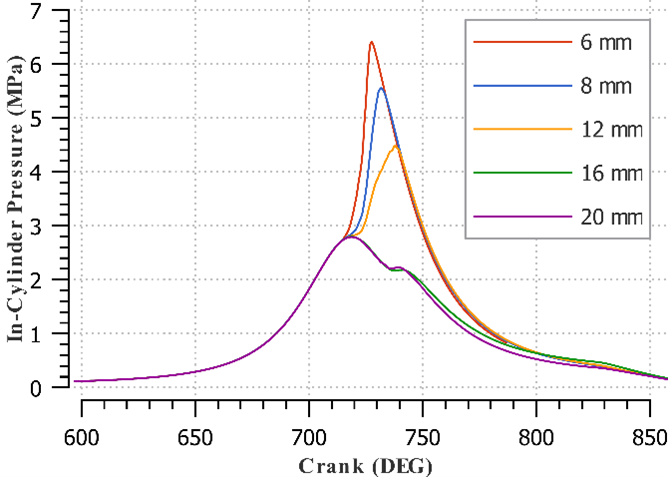
\includegraphics{plots and graphs/1.png}}
    \caption{In-cylinder pressure at different mesh configurations}
    \label{plt_1}
    \end{figure}

\subsection{Range selection}
The trends of in-cylinder pressure during normal and knocking combustion [13] is different from each other and it can be used to characterize knocking combustion. 
When the IST was earlier than 10\textsuperscript{0} after Inlet Valve Open (aIVO), a similar trend of intake-manifold pressure as with knocking combustion appeared (see Fig. 2). 
Conversely, when the IST is delayed beyond 20\textsuperscript{0} aIVO, the mixture fails to combust effectively. 
Only IST within the range 10\textsuperscript{0} aIVO - 20\textsuperscript{0} aIVO resulted in proper combustion. 
Therefore, IST of 10\textsuperscript{0} aIVO, 15textsuperscript{0} aIVO, and 20textsuperscript{0} aIVO were chosen to represent early, balanced, and delayed injection modes, respectively.

\begin{figure}[htbp]
    \centerline{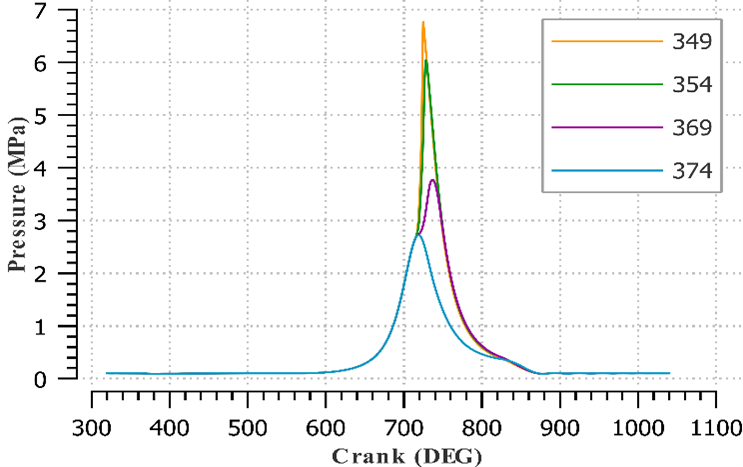
\includegraphics{plots and graphs/2.png}}
    \caption{In-cylinder pressure at different injection start times at VOT of 30\textsuperscript{0}}
    \label{plt_2}
    \end{figure}


\subsection{Trapped Mass}
Irrespective of the injection mode, a linear variation of trapped hydrogen mass with VOT could be observed (see Fig. 3). 
This can be understood by observing the variation of trapped mass with the crank angle at different VOTs, as shown in Fig. 4. 
When the VOT is reduced, Inlet Valve Close (IVC) is delayed (exhaust valve timing remained constant during the analysis). 
As a result, a larger fraction of the time when the inlet valve is open is affected by the upward push generated by the piston during the compression stroke. 
This is shown in the same figure as an extended duration of mass reduction after 540\textsuperscript{0}.

\begin{figure}[htbp]
    \centerline{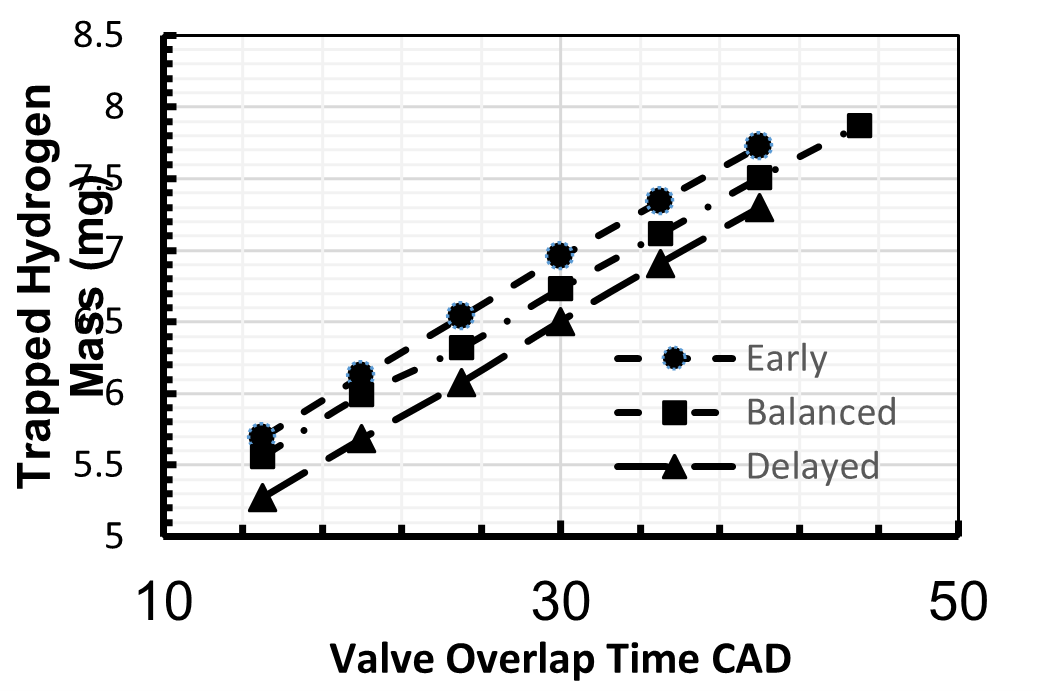
\includegraphics{plots and graphs/3.png}}
    \caption{Variation of trapped H\textsubscript{2} mass with VOT and Injection Mode.}
    \label{plt_3}
    \end{figure}


\begin{figure}[htbp]
    \centerline{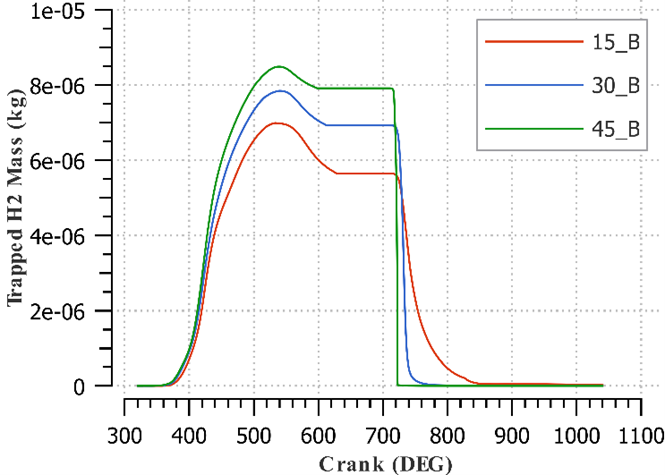
\includegraphics{plots and graphs/4.png}}
    \caption{Variation of trapped hydrogen mass at different valve times}
    \label{plt_4}
    \end{figure}

Furthermore, an increased VOT leads to an enhanced scavenging effect, which removes the exhaust residual gases from the chamber, thereby increasing the trapped mass. 
Further, when the injection is delayed relative to the IVO, only air flows into the cylinder for a few crank angles. 
This leads to a reduction in trapped mass with injection delay. 
This trend of reducing trapped mass with injection delay persists across every valve overlap within the selected range.\\

Another significant observation from the above variation is that a specific trapped mass can be attained through various combinations of valve and injection timings. 
Depending on other constraints, including combustion characteristics, engine performance, and the prevention of abnormal combustion events, it may be more beneficial to control one parameter over the other. 
However, to provide recommendations, further analysis is necessary.

\subsection{Local concentration}
As shown in Fig. 5, a high local concentration can form near the inlet valve during the starting of IVO. 
The influence of the injection mode and VOT is only dominant at low VOTs (see Fig.6). 
In contrast, at higher VOTs, it appears to be independent of both valve and injection timing.

\begin{figure}[htbp]
    \centerline{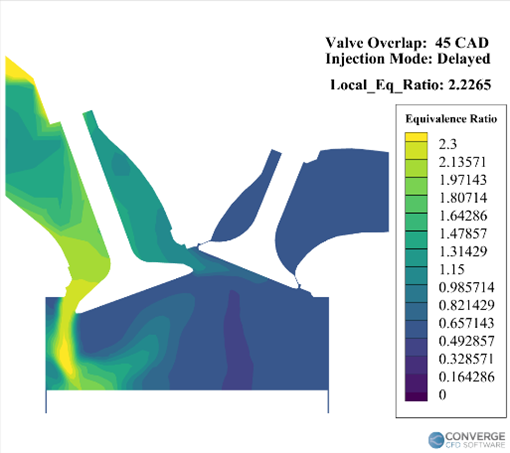
\includegraphics{plots and graphs/5.png}}
    \caption{Contours of localized equivalence ratio at VOT of 150 and early injection mode.}
    \label{plt_5}
    \end{figure}

Given that relatively higher local concentrations were recorded in all other cases, the only apparent method to reduce local concentrations seems to be a combination of reduced VOT and delayed injection mode.


\begin{figure}[htbp]
    \centerline{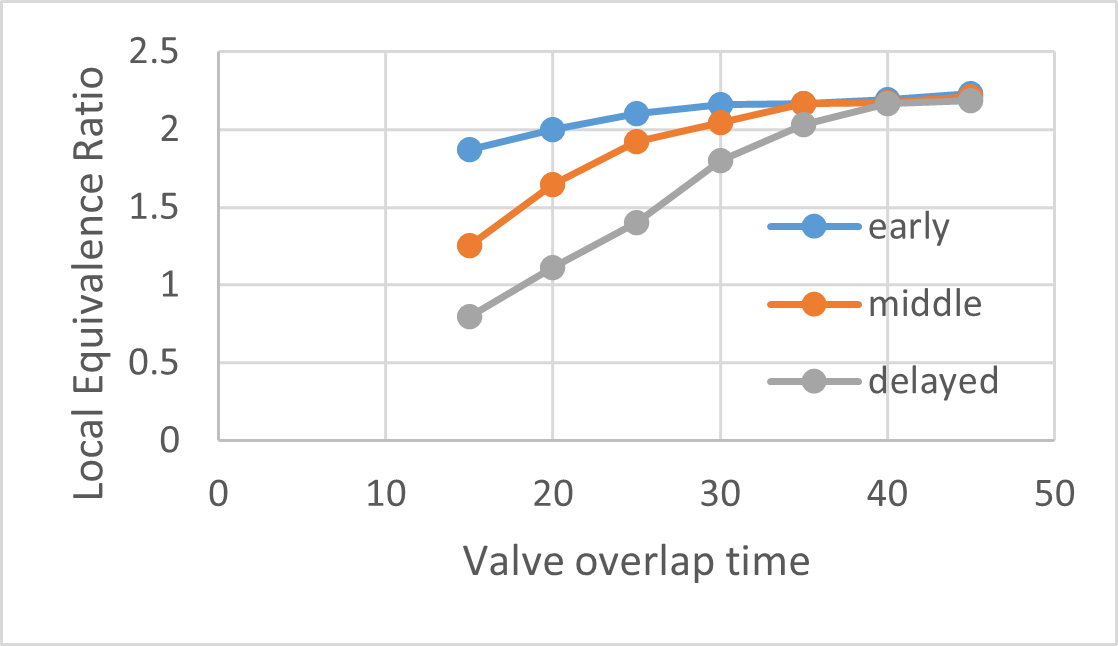
\includegraphics{plots and graphs/6.png}}
    \caption{Local concetration of hydrogen near valve seats}
    \label{plt_6}
    \end{figure}
    

\subsection{Combustion Characteristics}
Within the selected range, a similar knocking trend as explained in the section B with least in-cylinder pressure is observed when VOT was 40\textsuperscript{0} and early injection (see Fig 7). 
The recorded peak in-cylinder pressure was approximately 7 MPa. 
As intensive pressure rise is commonly used in the literature to characterize engine knock [13], operating conditions that resulted in peak in-cylinder pressures higher than 7 MPa can be classified as knocking combustions. 
On the other hand, improper combustion can be identified by a low-pressure rise. 
The combustion process when the VOT was 20textsuperscript{0} with balanced injection can be considered as improper combustion with the highest-pressure rise (see Fig. 7). 
The observed pressure was around 3 MPa.

\begin{figure}[htbp]
    \centerline{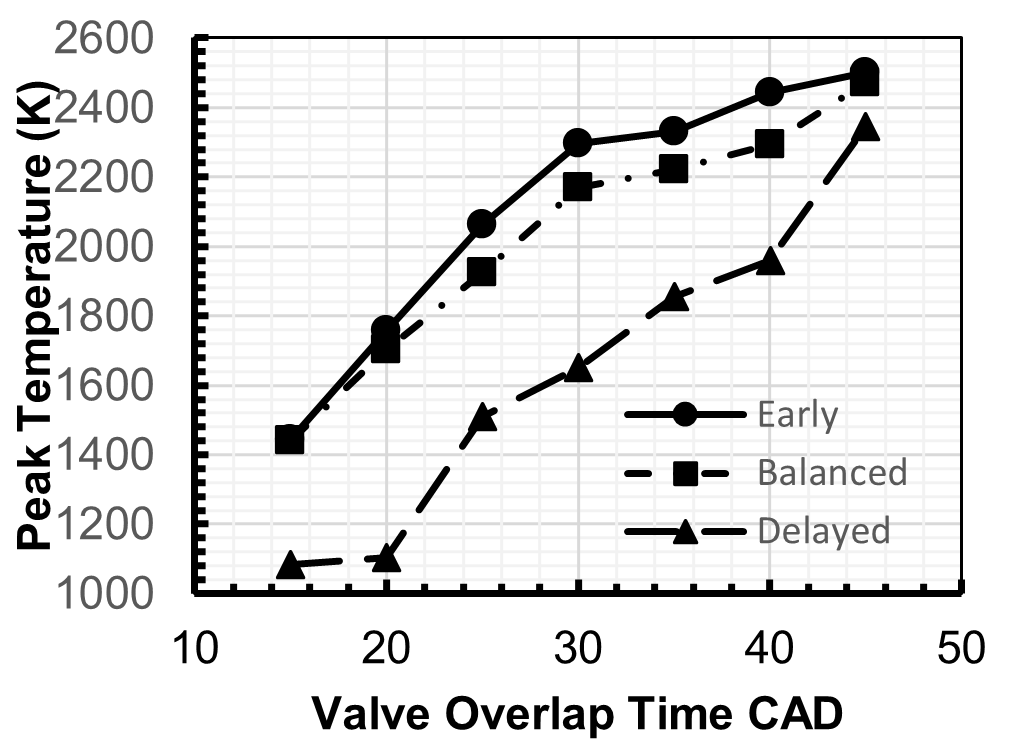
\includegraphics{plots and graphs/7.png}}
    \caption{Local concetration of hydrogen near valve seats}
    \label{plt_7}
    \end{figure}

Consequently, cases that resulted in pressures between 3 MPa and 7 MPa can be regarded as instances of proper combustion. 
These cases can be isolated in the peak in-cylinder pressure plot as illustrated in Fig. 9. 
Knocking combustion occurred in all cases with a VOT of 45\textsuperscript{0} and in those with VOTs exceeding 25\textsuperscript{0} during early injection. 
Improper combustion was observed in all cases with VOTs under 20\textsuperscript{0}, excluding the case with a VOT of 20\textsuperscript{0} during early injection.

\begin{figure}[htbp]
    \centerline{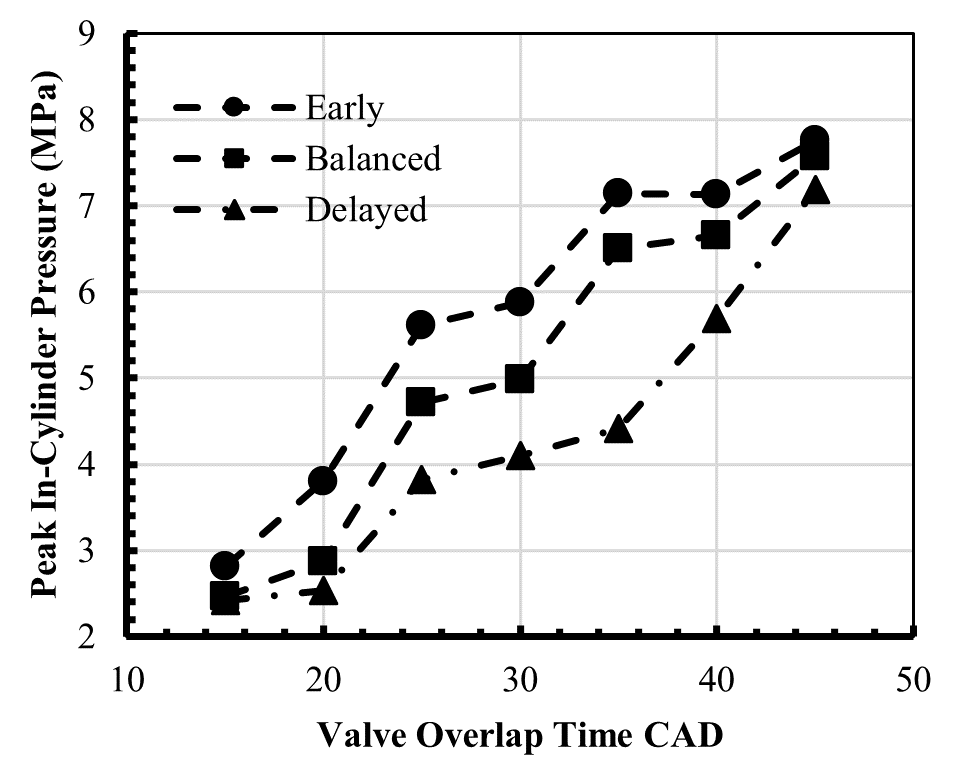
\includegraphics{plots and graphs/9.png}}
    \caption{Local concetration of hydrogen near valve seats}
    \label{plt_9}
    \end{figure}

A comparison of the trends of peak in-cylinder pressure and trapped hydrogen mass with VOT and injection mode revealed a strong positive correlation between them. 
The trapped hydrogen mass appeared to influence the combustion characteristics directly. 
Therefore, capturing the appropriate amount of hydrogen mass is crucial for the proper operation of the engine.

The peak in-cylinder temperature exhibited a similar variation to the peak in-cylinder pressure (see Fig. 10). 
High peak combustion temperatures consequently result in elevated local temperatures of engine components, including valves, spark plugs, and pistons, thereby increasing the risk of backfire. 
As explained by [3], both local concentration and temperature collectively influence the possibility of backfire. 
When both the combustion temperatures and local hydrogen concentrations are high, the possibility of backfire is at its maximum. 
Accordingly, cases with high VOT and early injection have the greatest potential for backfire within the studied range.


\begin{figure}[htbp]
    \centerline{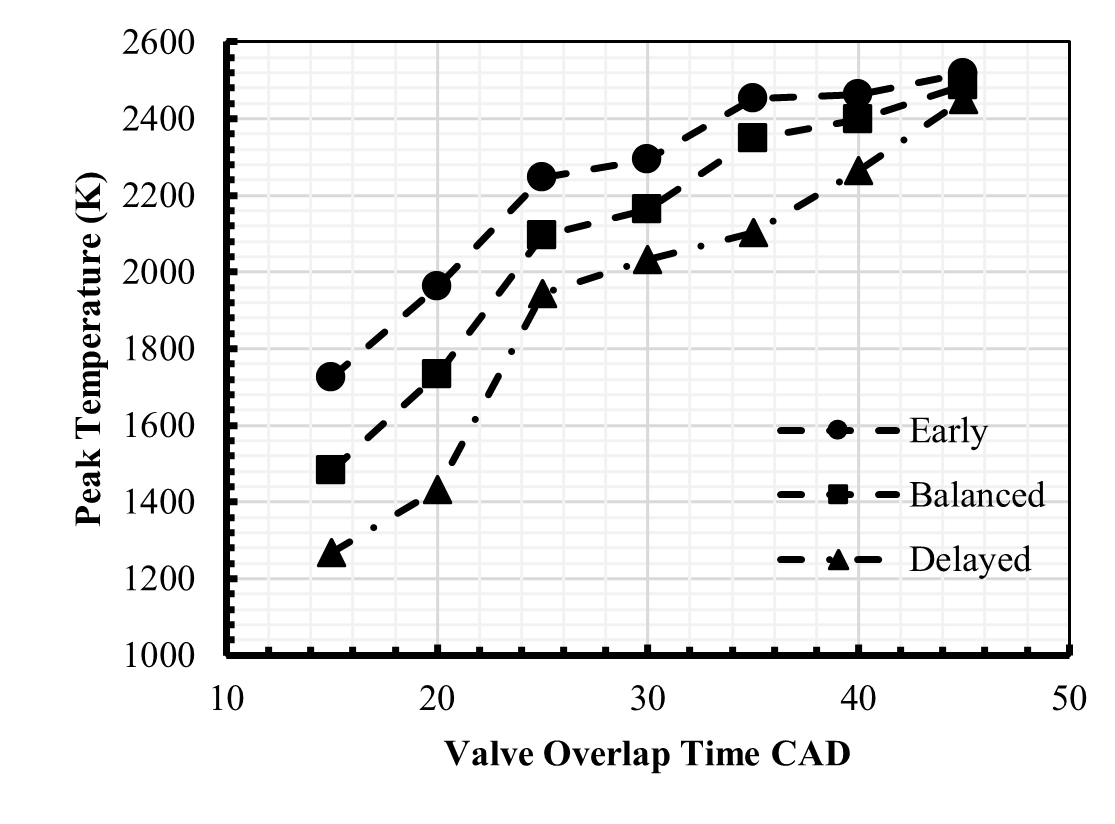
\includegraphics{plots and graphs/10.png}}
    \caption{Local concetration of hydrogen near valve seats}
    \label{plt_10}
    \end{figure}

\subsection{Performance}
IMEP as measure of engine performance, increases with VOT up to a certain point, then decreases for every injection mode (refer to Fig. 11). 
A rapid decrease in IMEP with low VOTs and injection delay could be attributed to the reduced trapped mass and subsequent improper combustion. 
Conversely, during knocking combustion, the pressure rise is sudden, leading to less effective work being produced. 
This sudden pressure rise acts as an impact load on the piston, failing to generate useful work. 
Hence, even though the in-cylinder pressure is high in these instances, the useful work is low. 
This phenomenon is reflected in the IMEP plot as a reduction of IMEP with high VOT, despite the high-pressure rise.

\begin{figure}[htbp]
    \centerline{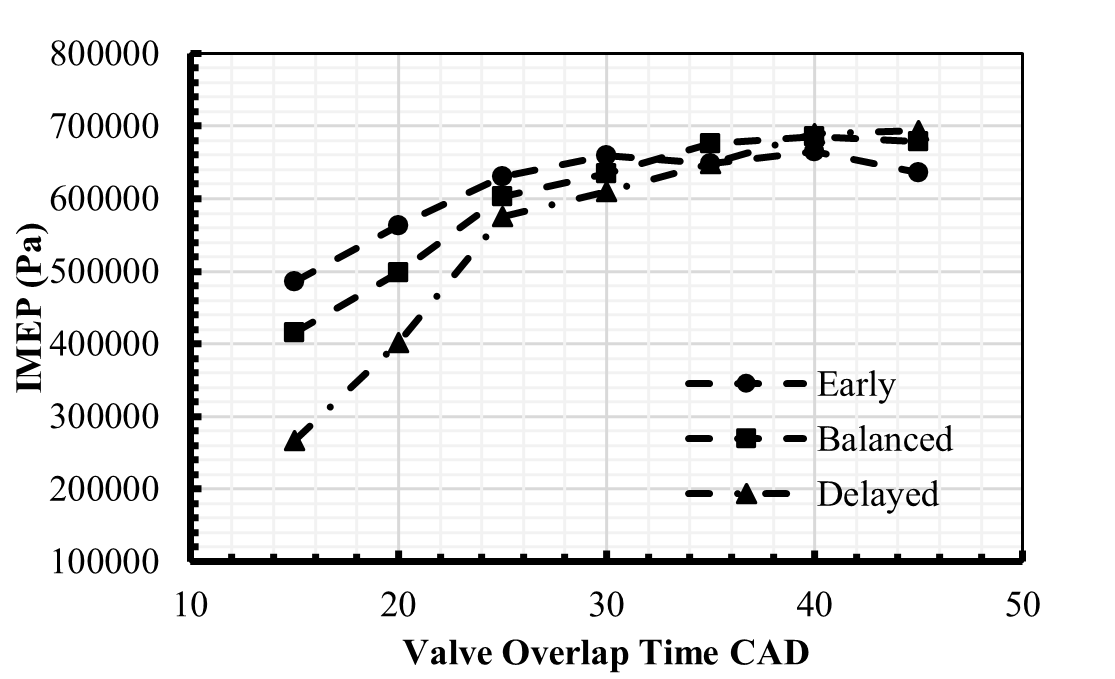
\includegraphics{plots and graphs/11.png}}
    \caption{Local concetration of hydrogen near valve seats}
    \label{plt_11}
    \end{figure}

\section{Conclusion}
\begin{itemize}
    \item A linear relationship was observed between the trapped hydrogen mass and VOT, regardless of the injection mode.
    \item The only noticeable method to decrease local concentrations appeared to be a reduction in VOT with a delayed injection mode.
    \item Knocking combustion was prevalent in all scenarios with a VOT of 450 and those with VOTs above 250 during early injection.
    \item Except for the case with a VOT of 200 during early injection, improper combustion was detected in all instances with VOTs less than 200. 
    \item IMEP rises with VOT up to a certain threshold, after which it decreases for all injection modes.
    \item The VOT for maximum IMEP showed an increase with injection delay.
\end{itemize}

\section{Future Works}
The primary focus of the current study was to examine the impact of valve and injection timing on combustion characteristics and engine performance. A more detailed analysis is required to understand the effects of these parameters on backfire. Future works in this study will involve identifying effective methods to mitigate backfire by altering valve and injection timings.

\section*{Acknowledgment}
We extend our heartfelt thanks to CONVERGE Science for providing the necessary commercial CFD code license for our research.

\begin{thebibliography}{00}
\bibitem{b1} L. Wang et al., “The effect of hydrogen injection parameters on the quality of hydrogen–air mixture formation for a PFI hydrogen internal combustion engine,” Int. J. Hydrog. Energy, vol. 42, no. 37, pp. 23832–23845, Sep. 2017, doi: 10.1016/j.ijhydene.2017.04.086.
\bibitem{b2} H. Yun, Z. Bu, Z. Yang, L. Wang, and B. Zhang, “Optimization of fuel injection timing and ignition timing of hydrogen fueled SI engine based on DOE-MPGA,” Int. J. Hydrog. Energy, vol. 48, no. 25, pp. 9462–9473, Mar. 2023, doi: 10.1016/j.ijhydene.2022.12.068.
\bibitem{b3} J. Duan, F. Liu, and B. Sun, “Backfire control and power enhancement of a hydrogen internal combustion engine,” Int. J. Hydrog. Energy, vol. 39, no. 9, pp. 4581–4589, Mar. 2014, doi: 10.1016/j.ijhydene.2013.12.175.
\bibitem{b4} X. Liu, F. Liu, L. Zhou, B. Sun, and H. Schock, “Backfire prediction in a manifold injection hydrogen internal combustion engine,” Int. J. Hydrog. Energy, vol. 33, no. 14, pp. 3847–3855, Jul. 2008, doi: 10.1016/j.ijhydene.2008.04.051.
\bibitem{b5} A. Menaa, M. S. Lounici, F. Amrouche, K. Loubar, and M. Kessal, “CFD analysis of hydrogen injection pressure and valve profile law effects on backfire and pre-ignition phenomena in hydrogen-diesel dual fuel engine,” Int. J. Hydrog. Energy, vol. 44, no. 18, pp. 9408–9422, Apr. 2019, doi: 10.1016/j.ijhydene.2019.02.123.
\bibitem{b6} C. Park, W. Park, Y. Kim, Y. Choi, and B. Lim, “Effect of Valve Timing and Excess Air Ratio on Torque in Hydrogen-Fueled Internal Combustion Engine for UAV,” Energies, vol. 12, no. 5, p. 771, Feb. 2019, doi: 10.3390/en12050771.
\bibitem{b7} T. C. Huynh, J. K. Kang, K. C. Noh, J. T. Lee, and J. A. Caton, “Controlling Backfire Using Changes of the Valve Overlap Period for a Hydrogen-Fueled Engine Using an External Mixture,” in ASME 2007 Internal Combustion Engine Division Fall Technical Conference, Charleston, South Carolina, USA: ASMEDC, Jan. 2007, pp. 243–251. doi: 10.1115/ICEF2007-1702.
\bibitem{b8} J. Lee, K. Lee, J. Lee, and B. Anh, “High power performance with zero NOx emission in a hydrogen-fueled spark ignition engine by valve timing and lean boosting,” Fuel, vol. 128, pp. 381–389, Jul. 2014, doi: 10.1016/j.fuel.2014.03.010.
\bibitem{b9} P. K. Senecal et al., “Multi-Dimensional Modeling of Direct-Injection Diesel Spray Liquid Length and Flam Lift-off Length using CFD an Parallel Detailed Chemistry”.
\bibitem{b10} M. Ó Conaire, H. J. Curran, J. M. Simmie, W. J. Pitz, and C. K. Westbrook, “A comprehensive modeling study of hydrogen oxidation,” Int. J. Chem. Kinet., vol. 36, no. 11, pp. 603–622, Nov. 2004, doi: 10.1002/kin.20036.
\bibitem{b11} V. Dhyani and K. A. Subramanian, “Fundamental characterization of backfire in a hydrogen fuelled spark ignition engine using CFD and experiments,” Int. J. Hydrog. Energy, vol. 44, no. 60, pp. 32254–32270, Dec. 2019, doi: 10.1016/j.ijhydene.2019.10.077.
\bibitem{b12} J. A. A. Yamin and M. H. Dado, “Performance simulation of a four-stroke engine with variable stroke-length and compression ratio,” Appl. Energy, vol. 77, no. 4, pp. 447–463, Apr. 2004, doi: 10.1016/S0306-2619(03)00004-7.
\bibitem{b13} M. U. Manzoor, M. Yosri, M. Talei, F. Poursadegh, Y. Yang, and M. Brear, “Normal and knocking combustion of hydrogen: A numerical study,” Fuel, vol. 344, p. 128093, Jul. 2023, doi: 10.1016/j.fuel.2023.128093.


\end{thebibliography}

\end{document}
